\documentclass[11pt]{article}

\usepackage[margin=1in]{geometry}
\usepackage[T1]{fontenc}
\usepackage{lmodern}
\usepackage{graphicx}
\usepackage{booktabs}
\usepackage{array}
\usepackage{caption}
\usepackage{subcaption}
\usepackage{enumitem}
\usepackage{hyperref}
\usepackage{xcolor}
\usepackage{pgfplots}

\pgfplotsset{compat=1.18}
\graphicspath{{repo/screenshots/}}

\title{End-to-End Deepfake Image Detector Report}
\author{}
\date{}

\begin{document}

\maketitle

\begin{abstract}
This report summarizes the deepfake image detector project end to end, from data collection through preprocessing, model design, evaluation, and final model selection. The write-up is based on the repository artifacts in \texttt{README.md}, \texttt{code/results/model\_eval.csv}, \texttt{code/results/v2b0\_history.csv}, and the training and testing notebooks. The strongest preserved model is an \textbf{EfficientNetV2-B0} classifier fine-tuned on the project dataset, reaching \textbf{0.9651 validation accuracy}, \textbf{0.9919 validation precision}, and \textbf{0.9824 validation AUC}. On the held-out test set, accuracy dropped to \textbf{0.8577}, which is consistent with the repository note that the test images include stronger manipulations than the training data.
\end{abstract}

\section{Project Objective}

The project goal is to classify images as \emph{real} or \emph{deepfake} using convolutional neural networks. The practical motivation is not only to build a high-accuracy classifier, but to identify a model that can be packaged as an out-of-the-box detector for realistic image manipulation settings.

The repository documents two main objectives:
\begin{enumerate}[leftmargin=1.5em]
    \item train several CNN-based models on a labeled real-vs-fake image dataset,
    \item compare architectures and keep the model with the best precision, accuracy, and overall validation behavior for deployment.
\end{enumerate}

\section{Data Collection}

The project uses the \textbf{OpenForensics} dataset, described in the repository as an open-source dataset of labeled real and fake images. The notebooks indicate a large-scale image classification setup:
\begin{itemize}[leftmargin=1.5em]
    \item approximately \textbf{140{,}002} training images,
    \item approximately \textbf{39{,}428} validation images,
    \item approximately \textbf{10.9k} test images.
\end{itemize}

Images are loaded from class directories with TensorFlow's \texttt{image\_dataset\_from\_directory}, using:
\begin{itemize}[leftmargin=1.5em]
    \item image size \textbf{256 x 256},
    \item batch size \textbf{64},
    \item binary real/fake labels.
\end{itemize}

The dataset selection was appropriate for this project because it already provided supervised labels and enough scale to compare lightweight custom CNNs with transfer-learning models.

\section{Data Cleaning and Preprocessing}

The repository notes that only light cleaning was required beyond organizing the dataset for supervised learning. The practical preprocessing pipeline used in the notebooks consists of:
\begin{enumerate}[leftmargin=1.5em]
    \item directory-based label loading for real and fake classes,
    \item resizing every image to \textbf{256 x 256},
    \item in-model rescaling / normalization,
    \item optional data augmentation for selected models, including flips and rotations,
    \item train / validation / test separation for fair comparison.
\end{enumerate}

This means the project is closer to a supervised image-classification pipeline than a heavy data-engineering project. The most important preprocessing design choice was standardization: every model received the same fixed image size and the same basic labeling structure, so architecture comparison remained meaningful.

\section{Model Families and Choices}

The repository states that \textbf{11 CNNs} were trained across local hardware and Google Colab, with roughly \textbf{35 hours} of total training. Two model families were explored:

\subsection{Sequential CNN Models}

These are custom convolutional models trained directly on the task. They provide:
\begin{itemize}[leftmargin=1.5em]
    \item a simple benchmark architecture,
    \item a tuned CNN variant after iterative improvement,
    \item a lower-compute baseline for comparison against transfer learning.
\end{itemize}

\subsection{EfficientNet-Based Models}

The stronger family used pretrained EfficientNet backbones. In the preserved results, the finalists include:
\begin{itemize}[leftmargin=1.5em]
    \item \textbf{cnn\_benchmark},
    \item \textbf{cnn\_tuned},
    \item \textbf{effnetv2L},
    \item \textbf{effnetv2b0}.
\end{itemize}

The testing notebook explicitly identifies \textbf{EfficientNetV2-B0} as the best choice among the preserved finalists. It is the smallest EfficientNetV2 model in the Keras API, initialized with ImageNet weights and then retrained on the deepfake classification dataset.

\section{Experimental Setup}

The training and evaluation workflow uses standard binary-classification metrics:
\begin{itemize}[leftmargin=1.5em]
    \item loss,
    \item accuracy,
    \item precision,
    \item recall,
    \item AUC.
\end{itemize}

These metrics were tracked during training and then compared on the validation set. The repository also preserves a final test-set evaluation for the selected EfficientNetV2-B0 model.

\section{Validation Results}

Table~\ref{tab:validation-results} summarizes the preserved validation results for the finalist models.

\begin{table}[htbp]
\centering
\caption{Validation metrics for preserved finalist models}
\label{tab:validation-results}
\begin{tabular}{lcccc}
\toprule
Model & Val.\ Loss & Val.\ Acc. & Val.\ Precision & Val.\ AUC \\
\midrule
cnn\_benchmark & 0.4216 & 0.8216 & 0.7723 & 0.9169 \\
cnn\_tuned     & 0.2601 & 0.9181 & 0.9142 & 0.9700 \\
effnetv2L      & 0.2864 & 0.8912 & 0.8875 & 0.9564 \\
effnetv2b0     & \textbf{0.1196} & \textbf{0.9651} & \textbf{0.9919} & \textbf{0.9824} \\
\bottomrule
\end{tabular}
\end{table}

Figure~\ref{fig:model-comparison} shows the same comparison as a validation-score chart.

\begin{figure}[htbp]
\centering
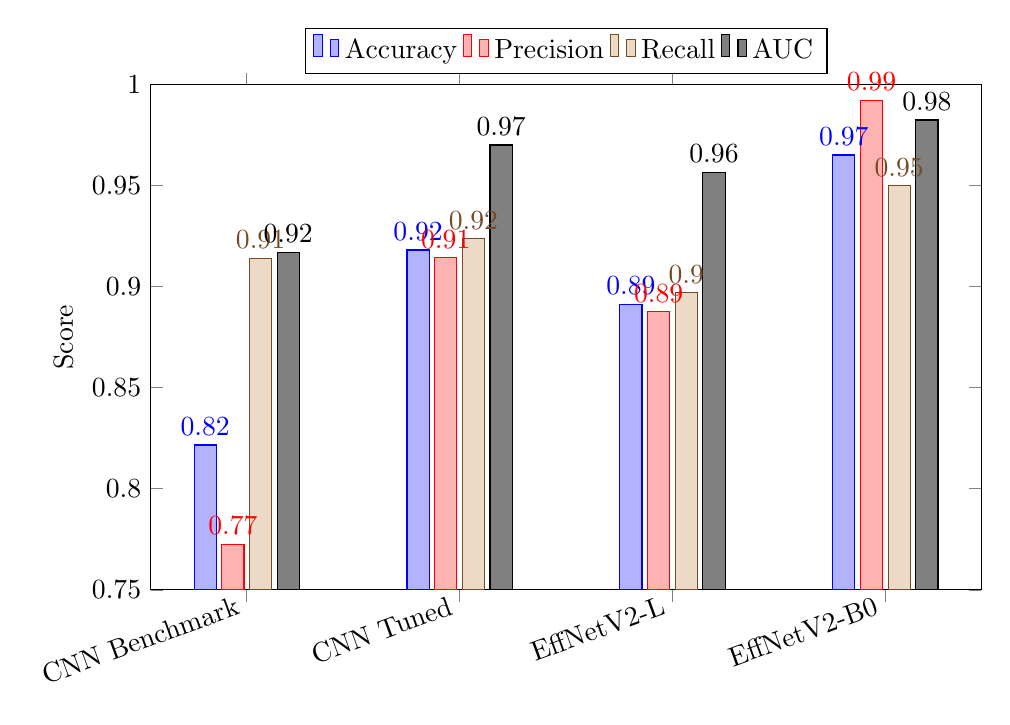
\begin{tikzpicture}
\begin{axis}[
    ybar,
    width=\textwidth,
    height=8cm,
    ymin=0.75,
    ymax=1.00,
    bar width=8pt,
    symbolic x coords={CNN Benchmark,CNN Tuned,EffNetV2-L,EffNetV2-B0},
    xtick=data,
    xticklabel style={rotate=20,anchor=east},
    ylabel={Score},
    legend style={at={(0.5,1.02)}, anchor=south, legend columns=-1},
    enlarge x limits=0.15,
    nodes near coords,
    nodes near coords align={vertical},
]
\addplot coordinates {(CNN Benchmark,0.8216) (CNN Tuned,0.9181) (EffNetV2-L,0.8912) (EffNetV2-B0,0.9651)};
\addplot coordinates {(CNN Benchmark,0.7723) (CNN Tuned,0.9142) (EffNetV2-L,0.8875) (EffNetV2-B0,0.9919)};
\addplot coordinates {(CNN Benchmark,0.9139) (CNN Tuned,0.9236) (EffNetV2-L,0.8969) (EffNetV2-B0,0.9498)};
\addplot coordinates {(CNN Benchmark,0.9169) (CNN Tuned,0.9700) (EffNetV2-L,0.9564) (EffNetV2-B0,0.9824)};
\legend{Accuracy,Precision,Recall,AUC}
\end{axis}
\end{tikzpicture}
\caption{Validation comparison across preserved finalist models}
\label{fig:model-comparison}
\end{figure}

The validation results lead to a clear conclusion:
\begin{itemize}[leftmargin=1.5em]
    \item the benchmark CNN establishes feasibility but underperforms the others,
    \item the tuned CNN is much stronger and shows that architecture refinement matters,
    \item EfficientNetV2-L does not beat the tuned CNN despite being larger,
    \item EfficientNetV2-B0 is the best tradeoff and best overall performer.
\end{itemize}

\section{Best Model Training Behavior}

The repository preserves the epoch history for the best model, EfficientNetV2-B0. The final recorded epoch reached:
\begin{itemize}[leftmargin=1.5em]
    \item training loss: \textbf{0.0052},
    \item training accuracy: \textbf{0.9985},
    \item validation loss: \textbf{0.1196},
    \item validation accuracy: \textbf{0.9651}.
\end{itemize}

\begin{figure}[htbp]
\centering

\includegraphics[width=0.82\textwidth]{v2b0_history.png}
\caption{Training history for EfficientNetV2-B0 preserved in the repository}
\label{fig:v2b0-history}
\end{figure}

Figure~\ref{fig:v2b0-history} shows stable convergence and strong validation accuracy, which is why the model became the recommended deployment candidate.

\section{Test Results}

The testing notebook evaluates EfficientNetV2-B0 on a held-out test dataset and reports:
\begin{itemize}[leftmargin=1.5em]
    \item test loss: \textbf{0.5126},
    \item test accuracy: \textbf{0.8577},
    \item test AUC: \textbf{0.9387},
    \item test precision: \textbf{0.9188},
    \item test recall: \textbf{0.7828}.
\end{itemize}

This drop from validation to test performance is one of the most important findings in the project. The repository notes that the test set contains a higher concentration of manipulated images, including blur, Gaussian noise, random-pixel removal, and other transformations meant to deceive deepfake detectors. That makes the test set harder and highlights the generalization problem.

\begin{figure}[htbp]
\centering
\begin{subfigure}[t]{0.48\textwidth}
    \centering
    
\includegraphics[width=\textwidth]{precision_recall.png}
    \caption{Precision-recall behavior}
\end{subfigure}
\hfill
\begin{subfigure}[t]{0.48\textwidth}
    \centering
    
\includegraphics[width=\textwidth]{v2b0_roc.png}
    \caption{ROC curve}
\end{subfigure}
\caption{Evaluation plots preserved in the repository for the selected model}
\label{fig:eval-curves}
\end{figure}

These plots show that the selected model remains useful on unseen test data, but not at the same level achieved on validation data. That is a meaningful result, because a detector intended for real deployment must be judged by its behavior on difficult examples, not only by its clean validation score.

\section{What the Project Actually Did}

From an end-to-end perspective, the project completed the following pipeline:
\begin{enumerate}[leftmargin=1.5em]
    \item collected a labeled real-vs-fake image dataset from OpenForensics,
    \item standardized the input pipeline to 256 x 256 images with TensorFlow dataset loaders,
    \item trained 11 CNN-based models across custom and transfer-learning architectures,
    \item preserved and compared finalist metrics,
    \item selected EfficientNetV2-B0 as the best deployment candidate,
    \item verified that harder test manipulations still reduce performance substantially.
\end{enumerate}

That last step matters. The project is not only a ``train a model and report accuracy'' exercise; it also identifies a practical limitation of the detector under stronger perturbations.

\section{Limitations and Improvement Opportunities}

The repository itself already points to the main weaknesses:
\begin{itemize}[leftmargin=1.5em]
    \item training data did not include enough additional image alterations beyond the deepfake manipulation itself,
    \item the harder test data exposes a generalization gap,
    \item stronger augmentation and longer training could likely improve robustness,
    \item more compute would allow broader backbone exploration and deeper hyperparameter tuning.
\end{itemize}

The most defensible next steps would be:
\begin{enumerate}[leftmargin=1.5em]
    \item add robustness-oriented augmentations during training,
    \item benchmark on multiple manipulated test subsets,
    \item preserve all 11-model comparison metrics in a single clean experiment log,
    \item calibrate the operating threshold depending on the target precision-recall tradeoff.
\end{enumerate}

\section{Conclusion}

The project successfully built an end-to-end deepfake image detection pipeline and produced a clear model-selection outcome. Among the preserved finalists, \textbf{EfficientNetV2-B0} is the best model: it achieves the strongest validation accuracy, precision, recall, and AUC, and it is therefore the correct recommendation for deployment from the current experiments.

At the same time, the test-set drop from \textbf{0.9651 validation accuracy} to \textbf{0.8577 test accuracy} is a valuable technical result. It shows that deepfake detection performance is sensitive to distribution shift and post-processing. The report therefore supports two conclusions at once: the project delivered a strong detector, and it also correctly identified robustness as the next problem to solve.

\end{document}
